\documentclass[tikz,border=6pt]{standalone}
\usetikzlibrary{arrows.meta,positioning}
\begin{document}
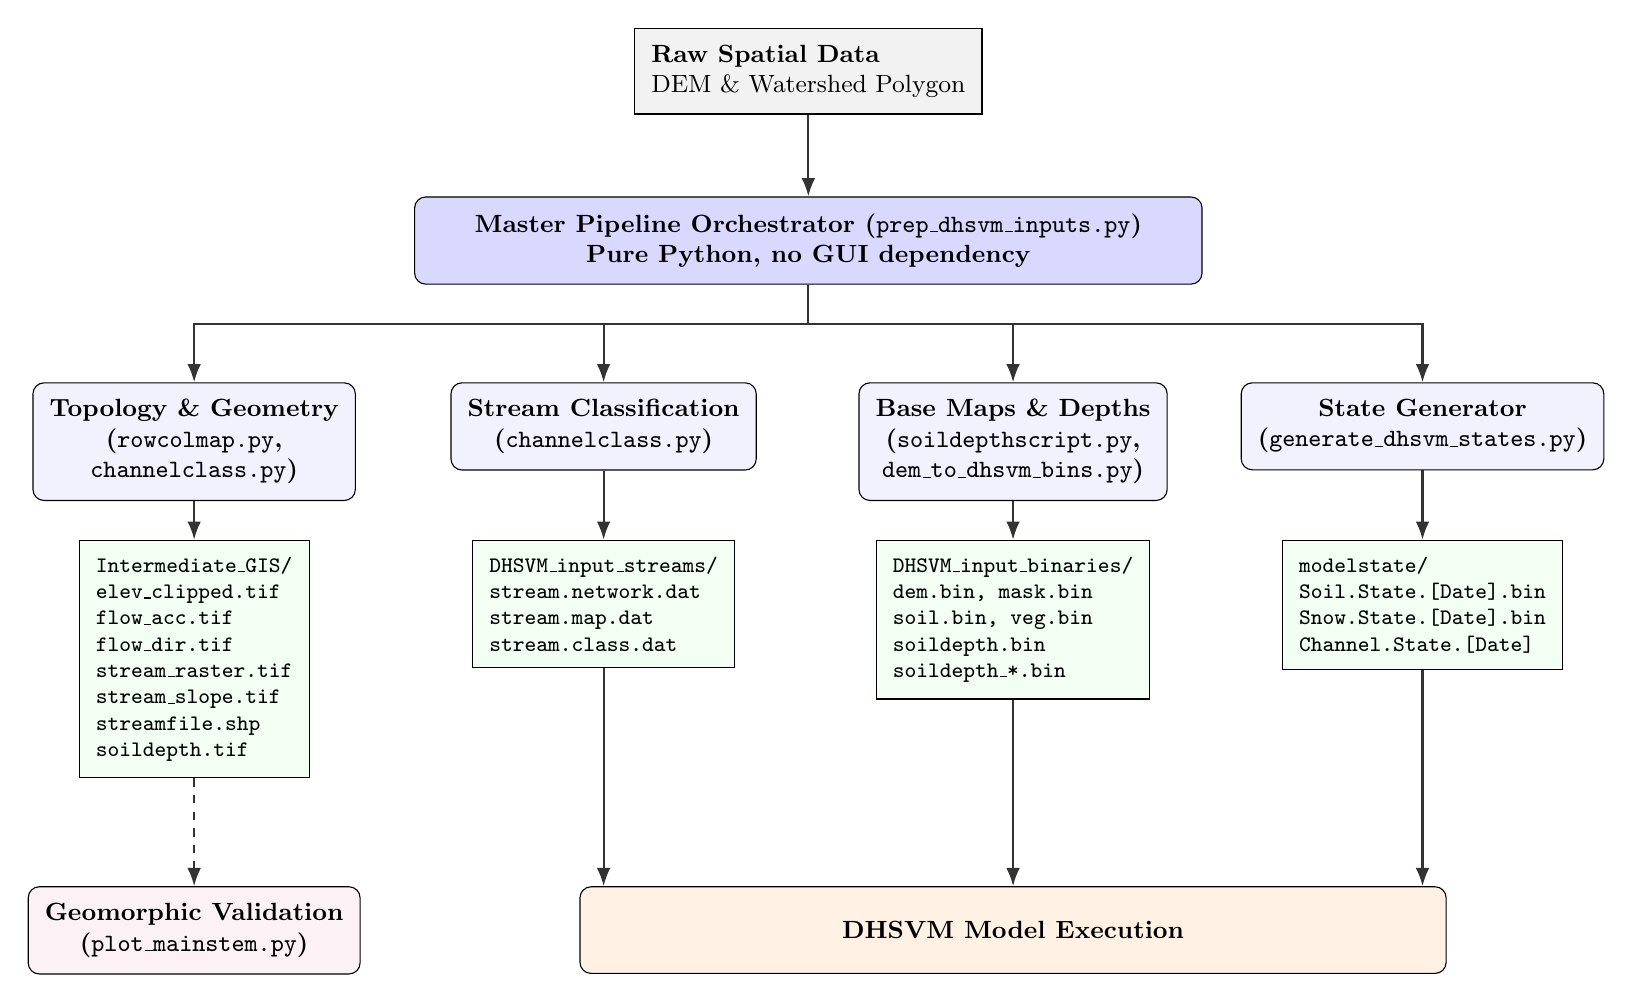
\begin{tikzpicture}[
  >=Latex,
  process/.style={rectangle, rounded corners, draw, align=center, fill=blue!5, font=\small\bfseries, inner sep=6pt, minimum height=1.1cm},
  data/.style={rectangle, draw, align=left, fill=green!5, font=\footnotesize\ttfamily, inner sep=6pt},
  validation/.style={rectangle, rounded corners, draw, align=center, fill=purple!5, font=\small\bfseries, inner sep=6pt, minimum height=1.1cm},
  arrow/.style={->, thick, draw=black!80}
]
\def\xGrass{-7.8}
\def\xStreams{-2.6}
\def\xBins{2.6}
\def\xStates{7.8}
\def\yMaster{0}
\def\yInputs{1.6}
\def\yLayerThree{-1.8}
\def\yLayerFour{-3.8}
\def\yLayerFive{-8.2}
\node[process, fill=blue!15, minimum width=10cm] (master) at (0, \yMaster) {Master Pipeline Orchestrator (\texttt{prep\_dhsvm\_inputs.py})\\Pure Python, no GUI dependency};
\node[data, fill=gray!10, font=\small, anchor=south] (inputs) at (0, \yInputs) {\textbf{Raw Spatial Data}\\DEM \& Watershed Polygon};
\node[process, anchor=north] (grass) at (\xGrass, \yLayerThree) {Topology \& Geometry\\(\texttt{rowcolmap.py},\\ \texttt{channelclass.py})};
\node[process, anchor=north] (streams) at (\xStreams, \yLayerThree) {Stream Classification\\(\texttt{channelclass.py})};
\node[process, anchor=north] (bins) at (\xBins, \yLayerThree) {Base Maps \& Depths\\(\texttt{soildepthscript.py},\\ \texttt{dem\_to\_dhsvm\_bins.py})};
\node[process, anchor=north] (states) at (\xStates, \yLayerThree) {State Generator\\(\texttt{generate\_dhsvm\_states.py})};
\node[data, anchor=north] (out_inter) at (\xGrass, \yLayerFour) {\textbf{Intermediate\_GIS/}\\elev\_clipped.tif\\flow\_acc.tif\\flow\_dir.tif\\stream\_raster.tif\\stream\_slope.tif\\streamfile.shp\\soildepth.tif};
\node[data, anchor=north] (out_stream) at (\xStreams, \yLayerFour) {\textbf{DHSVM\_input\_streams/}\\stream.network.dat\\stream.map.dat\\stream.class.dat};
\node[data, anchor=north] (out_bin) at (\xBins, \yLayerFour) {\textbf{DHSVM\_input\_binaries/}\\dem.bin, mask.bin\\soil.bin, veg.bin\\soildepth.bin\\soildepth\_*.bin};
\node[data, anchor=north] (out_state) at (\xStates, \yLayerFour) {\textbf{modelstate/}\\Soil.State.[Date].bin\\Snow.State.[Date].bin\\Channel.State.[Date]};
\node[process, fill=orange!10, minimum width=11cm, anchor=north] (dhsvm) at (\xBins, \yLayerFive) {DHSVM Model Execution};
\node[validation, anchor=north] (valid) at (\xGrass, \yLayerFive) {Geomorphic Validation\\(\texttt{plot\_mainstem.py})};
\draw[arrow] (inputs) -- (master);
\draw[arrow] (master.south) -- ++(0,-0.5) -| (grass.north);
\draw[arrow] (master.south) -- ++(0,-0.5) -| (streams.north);
\draw[arrow] (master.south) -- ++(0,-0.5) -| (bins.north);
\draw[arrow] (master.south) -- ++(0,-0.5) -| (states.north);
\draw[arrow] (grass) -- (out_inter);
\draw[arrow] (streams) -- (out_stream);
\draw[arrow] (bins) -- (out_bin);
\draw[arrow] (states) -- (out_state);
\draw[arrow, dashed] (out_inter) -- (valid);
\draw[arrow] (out_stream) -- (out_stream |- dhsvm.north);
\draw[arrow] (out_bin) -- (out_bin |- dhsvm.north);
\draw[arrow] (out_state) -- (out_state |- dhsvm.north);
\end{tikzpicture}
\end{document}
